\documentclass[calculator,datasheet,handbook,solutions]{exam}
% The full list of class options are
% calculator : Allows approved calculator use.
% datasheet : Adds a note that data sheet are attached to the exam.
% handbook : Allows the use of the engineering handbook.
% resit : Adds the resit markings to the paper.
% sample : Adds conspicuous SAMPLE markings to the paper
% solutions : Uses the contents of \solution commands (and \solmarks) to generate a solution file

\usepackage{array}
\usepackage{multirow}
\usepackage{pdfpages}
\usepackage[hidelinks]{hyperref}

\examtime{2~pm -- 5~pm}%
\examdate{13}{12}{2017}%
\examformat{Candidates should attempt \textit{all} questions.}

\newtoggle{3030paper}

%This changes the mode from EX3030 to EM40JN
\toggletrue{3030paper}
%\togglefalse{3030paper}

\iftoggle{3030paper}{
  \coursecode{EX3030}%
  \coursetitle{Heat, Mass, \& Momentum Transfer}%
}{
  \coursecode{EM40JN}%
  \coursetitle{Heat and Momentum Transfer}%
}

\begin{document}
%%%%%%%%%%%%%%%%%%%%%%%%%%%%%%%%%%%%%%%%%%%%%%%%%%%%%%%%%%%%%%%%%%%%%%%%%%%%%%%% 
%%%%%%%%%%%%%%%%%%%%%%%%%%%%%%%%%%%%%%%%%%%%%%%%%%%%%%%%%%%%%%%%%%%%%%%%%%%%%%%%

%%%
%%%  December Diet: Q01
%%%
\begin{question}
  \begin{enumerate}
    \item Consider a large aluminium plate of thickness 0.12 m with initial uniform temperature of 85$^{\circ}$C. Suddenly, the temperature of one of the faces is lowered to 20$^{\circ}$C, while the other face is perfectly insulated. Assuming that the plate can be modelled as a 1D problem, the following thermal energy conservative equation can be used,
    \begin{displaymath}
      \rho C_{p}\frac{\partial T}{\partial t} = \kappa \frac{\partial^{2} T}{\partial x^{2}} + \mathcal{S},
    \end{displaymath}
    where $\rho$, $C_{p}$, $t$ are density, heat capacity and time, respectively. $\kappa$ and $\mathcal{S}$ are thermal conductivity coefficient and source term.  Using the finite difference method (FDM) with spatial $\left(\Delta  x\right)$ and temporal $\left(\Delta t\right)$ increments of 0.03 m and 300 s, respectively, 
  \begin{enumerate}[a)]
     \item Determine the number of nodes necessary to discretise the problem;~\marks{1}
       \solution{For a length $L=0.12$ m and spatial increment $\Delta  x = 30\times 10^{-3}$ m,~\solmarks{1}
         \begin{displaymath}
           \Delta x = \frac{L}{M-1} \;\;\Longrightarrow\;\; M = 5\text{ nodes}
          \end{displaymath}

         }
     \item Describe the boundary and initial conditions for this problem;~\marks{3} 
       \solution{ For 5 nodes, $i=0,\cdots,4$
         \begin{enumerate}[(i)]
            \item Boundary conditions:
              \begin{itemize}
                 \item Dirichlet BC at $x = L =$ 0.12 m;~\solmarks{1}
                     \begin{displaymath}
                        T\left(x=L,t\right) = T_{4}^{j} = 20^{\circ}\text{C},\;\;\;\left(j=0,1,\cdots\right)
                     \end{displaymath}
                 \item Adiabatic plane at $x=0$ can be treated as a symmetric plane, i.e.,~\solmarks{1}
                     \begin{displaymath}
                        T_{i+1}^{j} = T_{i-1}^{j} \;\;\text{ for } i=0\;\;\Longrightarrow\;\; T_{1}^{j}=T_{-1}^{j}
                     \end{displaymath}
              \end{itemize}
            \item Initial condition: the plate has uniform temperature of 85$^{\circ}$C, i.e.,~\solmarks{1}
              \begin{displaymath}
                T\left(x<L,t=0s\right) = T_{i}^{0} = 85^{\circ}\text{C},\;\;\;\left(i=0,1,2,3\right)
              \end{displaymath}
         \end{enumerate}
         }
     \item Determine the temperature distribution of the plate at $t = 10$ minutes using the FDM,~\marks{12}
       \solution{ The discretised thermal energy equation,
          \begin{displaymath}
             \rho C_{p}\frac{T_{i}^{j+1}-T_{i}^{j+1}}{\Delta t} = \kappa \frac{T_{i+1}^{j}-2T_{i}^{j}+T_{i-1}^{j}}{\left(\Delta x\right)^{2}} + \mathcal{S}_{i}^{j},
          \end{displaymath}
          can be re-arranged to
          \begin{displaymath}
            \frac{\rho C_{p}}{\kappa} \frac{\left(\Delta x\right)^{2}}{\Delta t} \left(T_{i}^{j+1}-T_{i}^{j+1}\right) =  \left(T_{i+1}^{j}-2T_{i}^{j}+T_{i-1}^{j}\right) + \frac{\left(\Delta x\right)^{2}}{\kappa}\mathcal{S}_{i}^{j}.
          \end{displaymath}
          Defining the mesh Fourier number,
          \begin{displaymath}
            \tau = \frac{\alpha \Delta t}{\left(\Delta x\right)^{2}}
          \end{displaymath}
          and the thermal diffusivity, $\left(\alpha=\kappa\rho^{-1}C_{p}^{-1}\right)$,
          \begin{displaymath}
            T_{i}^{j+1} = T_{i}^{j} + \tau\left(T_{i+1}^{j} - 2T_{i}^{j}+T_{i-1}^{j}\right) + \frac{\tau\left(\Delta x\right)^{2}}{\kappa}\mathcal{S}_{i}^{j}.
          \end{displaymath}
          For this problem, the source term is null, $\mathcal{S}_{i}^{j}=0$, ~\solmarks{1}
          \begin{displaymath}
            T_{i}^{j+1} = T_{i}^{j} + \tau\left(T_{i+1}^{j} - 2T_{i}^{j}+T_{i-1}^{j}\right).
          \end{displaymath}
          The first step to solve FDM problems is to check if the stability criteria is met, i.e., $\tau \le 0.5$\solmarks{1}
          \begin{displaymath}
            \tau = \frac{\alpha \Delta t}{\left(\Delta x\right)^{2}} = 0.5 \;\;\text{ with }\;\;\Delta t = 300\text{ s}.
          \end{displaymath}
          Boundary and initial conditions are:
          \begin{displaymath}
            \begin{cases}
               \text{BC1: } T_{4}^{j} = 20, & j = 0,1,\cdots \\
               \text{BC2: } T_{i}^{j} = T_{-1}^{j}, & j = 0,1,\cdots \\
               \text{IC: } T_{i}^{0} = 85, & i = 0,\cdots, 3 
            \end{cases}
          \end{displaymath}
          Now solving the problem for $j=0,1,2$
          \begin{description}
            \item[j=0] $\rightarrow\;\;T_{i}^{j+1}=T_{i}^{1}$ $\left(t=300 s\right)$:\solmarks{5}
              \begin{displaymath}
                \begin{cases}
                   i=0, & T_{0}^{1} = T_{0}^{0} + \tau\left(T_{1}^{0}-2T_{0}^{0}+T_{-1}^{0}\right) = 85 \\
                   i=1, & T_{1}^{1} = T_{1}^{0} + \tau\left(T_{2}^{0}-2T_{1}^{0}+T_{0}^{0}\right) = 85 \\
                   i=2, & T_{2}^{1} = T_{2}^{0} + \tau\left(T_{3}^{0}-2T_{2}^{0}+T_{1}^{0}\right) = 85 \\
                   i=3, & T_{3}^{1} = T_{3}^{0} + \tau\left(T_{4}^{0}-2T_{3}^{0}+T_{2}^{0}\right) = 52.50 \\
                   i=4, & T_{4}^{1} = 20 \\
                \end{cases}
              \end{displaymath}
              
            \item[j=1] $\rightarrow\;\;T_{i}^{j+1}=T_{i}^{2}$ $\left(t=600 s\right)$:\solmarks{5}
              \begin{displaymath}
                \begin{cases}
                   i=0, & T_{0}^{2} = T_{0}^{1} + \tau\left(T_{1}^{1}-2T_{0}^{1}+T_{-1}^{1}\right) = 85 \\
                   i=1, & T_{1}^{2} = T_{1}^{1} + \tau\left(T_{2}^{1}-2T_{1}^{1}+T_{0}^{1}\right) = 85 \\
                   i=2, & T_{2}^{2} = T_{2}^{1} + \tau\left(T_{3}^{1}-2T_{2}^{1}+T_{1}^{1}\right) = 68.75 \\
                   i=3, & T_{3}^{2} = T_{3}^{1} + \tau\left(T_{4}^{1}-2T_{3}^{1}+T_{2}^{1}\right) = 52.50 \\
                   i=4, & T_{4}^{2} = 20 \\
                \end{cases}
              \end{displaymath}
          \end{description}
          
         }
  \end{enumerate}
    Thermal diffusivity $\left(\alpha=\kappa\rho^{-1}C_{p}^{-1}\right)$ of the plate is 1.5$\times$10$^{-6}$ m$^{2}$.s$^{-1}$. The discretised form of the thermal energy equation is
    \begin{displaymath}
      \rho C_{p}\frac{T_{i}^{j+1}-T_{i}^{j+1}}{\Delta t} = \kappa \frac{T_{i+1}^{j}-2T_{i}^{j}+T_{i-1}^{j}}{\left(\Delta x\right)^{2}} + \mathcal{S}_{i}^{j},
    \end{displaymath}
    where $i$ and $j$ are spatial and temporal indices.

   \item A double-pipe (shell-and-tube) heat exchanger is constructed of a stainless steel ($\kappa=$ 15.1 W/(m.$^{\circ}$C) inner tube of inner diameter D$_{i}=$ 1.5 cm and outer diameter D$_{o}=$ 1.9 cm and an outer shell of inner diameter 3.2 cm. The convective heat transfer coefficient is h$_{i}=$ 800 W/(m$^{2}.^{\circ}$C) on the inner surface of the tube and h$_{o}=$ 1200 W/(m$^{2}.^{\circ}$C) on the outer surface. For a fouling factor R$_{f,i}=$ 0.0004 m$^{2}.^{\circ}$C/W on the tube side and R$_{f,o}=$ 0.0001 m$^{2}.^{\circ}$C/W on the shell side, determine:%%% Slide (Cengel Example 13.1)
\begin{enumerate}
   \item The thermal resistance of the heat exchanger per unit length $\left(\text{in }^{\circ}\text{C/W}\right)$ and; \marks{3}
     \solution{ The total thermal resistance, $R$, of the heat exchanger through the pipes per unit length is\solmarks{1}
       \begin{displaymath}
           R = \frac{1}{h_{i}A_{i}} + \frac{R_{fi}}{A_{i}} + \frac{\ln{\left(\frac{D_{0}}{D_{i}}\right)}}{2\pi\kappa L} + \frac{R_{f0}}{A_{0}} + \frac{1}{h_{0}A_{0}},
       \end{displaymath}
     where $A_{i}=0.04712$ m$^{2}$ and $A_{0}=0.5969$ m$^{2}$, resulting in $\mathbf{R = 5.3145\times 10^{-2\circ}}${\bf C.W}$^{-1}$\solmarks{2}}
       
   \item The overall heat transfer coefficients, U$_{i}$ and U$_{o}$ $\left(\text{in W/}\left(\text{m}^{2}.^{\circ}\text{C}\right)\right)$ based on the inner and outer surface areas of the tube, respectively.\marks{6}
     \solution{The overall heat transfer coefficient based on the inner and the outter surface areas of the tube per length are
       \begin{displaymath}
         R = \frac{1}{UA} = \frac{1}{U_{i}A_{i}} = \frac{1}{U_{0}A_{0}},
       \end{displaymath}
       thus for $U_{i}$\solmarks{3}
       \begin{displaymath}
         U_{i} = \frac{1}{R A_{i}} = 399.3303 \frac{\text{W}}{\text{m}^{2}.^{\circ}\text{C}}
       \end{displaymath}
       and for $U_{0}$\solmarks{3}
       \begin{displaymath}
         U_{0} = \frac{1}{R A_{0}} = 315.2461 \frac{\text{W}}{\text{m}^{2}.^{\circ}\text{C}}
       \end{displaymath}
       }
\end{enumerate}


  \end{enumerate}
  
\end{question}

\pagebreak
%%%
%%%  December Diet: Q02
%%%
  
\begin{question}

  \begin{enumerate}[1.]
    \item A new material is to be developed for bearing balls in a new rolling-element bearing. For annealing (heat treatment) each bearing ball, a sphere of radius $r_{o} =$ 5 mm, is heated in a furnace until it reaches to the equilibrium temperature of the furnace at 400$^{\circ}$C. Then, it is suddenly removed from the furnace and subjected to a two-step cooling process.
       \begin{description}
           \item[Stage 1:] Cooling in an air flow of 20$^{\circ}$C for a period of time $t_{\text{air}}$ until the center temperature reaches 335$^{\circ}$C. For this situation, the convective heat transfer coefficient of air is assumed constant and equal to $h =$ 10 W/(m$^{2}$.K). After the sphere has reached this specific temperature, the second step is initiated. 
           \item[Stage 2:] Cooling in a well-stirred water bath at 20$^{\circ}$C, with a convective heat transfer coefficient of water $h =$ 6000 W/(m$^{2}$.K). 
       \end{description}
       The thermophysical properties of the material are $\rho =$ 3000 kg/m$^{3}$, $\kappa =$ 20 W/(m.K), $C_{p} =$ 1000 J/(kg.K). Determine:
        \begin{enumerate}%[(a)]
           \item The time $t_{\text{air}}$ required for {\it Stage 1} of the annealing process to be completed;\marks{5}
             \solution{ The first step is to check if the lumped-capacitance method can be used:\solmarks{1}
               \begin{displaymath}
                 \mathbf{Bi =} \frac{h L_{c}}{\kappa} = \mathbf{8.33\times 10^{-4}}
               \end{displaymath}
               As $\mathbf{Bi < 0.1}$~\solmarks{1}, the lumped-capacitance method can be used in this stage, i.e., temperature changes uniformily throughout the sphere,\solmarks{3}
                 \begin{eqnarray}
                   && \frac{T(t)-T_{\infty}}{T_{0}-T_{\infty}} = \exp{\left[-\frac{h}{L_{c}\rho C_{p}}t\right]} \nonumber \\
                   && \frac{335-20}{400-20} = \exp{\left[-\frac{10 t}{\frac{5\times 10^{-3}}{3}\times 3000 \times 1000}\right]} \;\;\Rightarrow \;\; \mathbf{t = 93.80 \text{ s}} \nonumber
                 \end{eqnarray}     
             }
           \item The time $t_{\text{water}}$ required for {\it Stage 2} of the annealing process during which the center of the sphere cools from 335$^{\circ}$C (the condition at the completion of {\it Stage 1}) to 50$^{\circ}$C.\marks{6}
             \solution{ Checking if the lumped-capacitance method can be used:
                \begin{displaymath}
                   \mathbf{Bi = \frac{h L_{c}}{\kappa} = 0.5 > 0.1},
                \end{displaymath}
                therefore the {\bf lumped-capacitance method can not be used}~\solmarks{1}. In order to use the Tables for the analytical solution, we need to calculate the $Bi$ number based on $r_{0}$, 
                \begin{displaymath}
                   Bi = \frac{hr_{0}}{\kappa}=1.5
                \end{displaymath}
                From the Table with coefficients for the one-term approximate solution of 1D transient conduction in spheres, we can obtain $\mathbf{\lambda_{1} = 1.7998}$ and $\mathbf{A_{1} = 1.3763}$\solmarks{2} to be applied into
                \begin{displaymath}
                   \theta_{\text{centre}} = \frac{T_{0}-T_{\infty}}{T_{i}-T_{\infty}} = \frac{50-20}{335-20}=A_{1}\exp{\left[-\lambda_{1}^{2}\tau\right]},
                \end{displaymath}
                where $\tau=\alpha t.r_{0}^{-2}$ with $\mathbf{\alpha=\kappa.\left(\rho C_{p}\right)^{-1} = 6.67\times 10^{-6} \text{ m}^{2}.\text{s}^{-1}}$.\solmarks{1}
          
                Solving the equation above results in $\mathbf{\tau = 0.8245}$\solmarks{1}, and $t$ is obtained from the Fourier number,\solmarks{1}
                  \begin{displaymath}
                    \mathbf{\tau =} \frac{\alpha t}{r_{0}^{2}} \;\;\Rightarrow \;\; \mathbf{t = 3.09}\text{ {\bf s}}
                  \end{displaymath}        
             }
        \end{enumerate}
        
    \item Water at the rate of 68 kg/min is heated from 35 to 75$^{\circ}$C by an oil having a specific heat of 1.9 kJ/(kg.$^{\circ}$C). The fluids are used in a counterflow double-pipe HE, and the oil enters the exchanger at 110$^{\circ}$C and leaves at 75$^{\circ}$C. The overall heat-transfer coefficient is 320 W/(m$^{2}.^{\circ}$C). Given heat capacity of water (at constant pressure) of 4.18 kJ/(kg.$^{\circ}$C),
\begin{enumerate}[(a)]
   \item Calculate the HE area;\marks{9}
     \solution{The total heat transfer can be obtained from~\solmarks{2}
       \begin{displaymath}
         Q = \dot{m}_{w}C_{p,w}\Delta T_{w} = 189.49\text{ kJ.s}^{-1}.
       \end{displaymath}
       And the heat exchange surface area can be calculated from
       \begin{displaymath}
         Q = U A \Delta T_{lm},
       \end{displaymath}
       where $U= 320$ W.m$^{-2}.^{\circ}$C$^{-1}$ and~\solmarks{5}
       \begin{displaymath}
         \Delta T_{lm} = \frac{\left(T_{h,in}-T_{c,out}\right)-\left(T_{h,out}-T_{c,in}\right)}{\ln{\frac{T_{h,in}-T_{c,out}}{T_{h,out}-T_{c,in}}}} = 37.44^{\circ}\text{C},
       \end{displaymath}
       thus~\solmarks{2}
       \begin{eqnarray}
         Q &=& U A \Delta T_{lm} =  189.49\text{ kJ.s}^{-1} \nonumber \\
         A &=& 15.82\text{ m}^{2} \nonumber
       \end{eqnarray}       
     }
   \item Now assume that the heat exchanger is a shell-and-tube with water making one shell pass and the oil making two tube passes. Calculate the area of the new heat exchanger. Assume that the overall heat-transfer coefficient remains the same.\marks{5}
     \solution{For cross-flow and multi-pass shell-and-tubes heat exchangers,
       \begin{displaymath}
         Q = U A F \Delta T_{lm}. 
       \end{displaymath}
       From Fig. 10.8 with,~\solmarks{2}
       \begin{displaymath}
         \begin{cases}
           R = \frac{T_{c,in}-T_{c,out}}{T_{h,out}-T_{h,in}} = 1.1429, & \\
           P = \frac{T_{h,out}-T_{h,in}}{T_{c,in}-T_{h,in}} = 0.4667, & \\
         \end{cases}
       \end{displaymath}
       leads to $F\sim 0.8$~\solmarks{1} and~\solmarks{2}
       \begin{displaymath}
         Q = U A F \Delta T_{lm} \;\;\Longrightarrow\;\; A = 19.77\text{ m}^{2}
       \end{displaymath}
     }
\end{enumerate}

  \end{enumerate}
  
\end{question}

\pagebreak
%%%
%%%  Resit Diet: Q01
%%%
\begin{question}
  \begin{enumerate}
      \item  Hot oil is to be cooled in a double-tube counter-flow heat exchanger. The copper inner tubes have diameter of 2 cm and negligible thickness. The inner diameter of the outer tube (shell) is 3 cm. Water flows through the tube at a rate of 0.5 kg.s$^{-1}$, and the oil through the shell at a rate of 0.8 kg.s$^{-1}$. Taking the average temperatures of the water and the oil to be 45$^{\circ}$C and 80$^{\circ}$C, respectively, determine the overall heat transfer coefficient of this heat exchanger. Given, 
         \begin{enumerate} 
             \item Water at 45$^{\circ}$C: $\rho=990$ kg.m$^{-3}$, $\kappa=0.637$ W.(m.K)$^{-1}$, $Pr=3.91$, $\nu=\mu/\rho=0.602\times 10^{-6}$ m$^{2}$.s$^{-1}$; 
             \item Oil at 80$^{\circ}$C: $\rho=852$ kg.m$^{-3}$, $\kappa=0.138$ W.(m.K)$^{-1}$, $Pr=490$, $\nu=37.5\times 10^{-6}$ m$^{2}$.s$^{-1}$.
         \end{enumerate}
         The overall heat transfer coefficient can be expressed as,
           \begin{displaymath}
             U^{-1} = h_{i}^{-1} + h_{0}^{-1}
           \end{displaymath}
         The inner convective heat transfer coefficient, $h_{i}$, can be obtained from
         \begin{displaymath}
                Nu = \frac{h_{i}D_{h}}{\kappa} =
                     \begin{cases}
                         4.36  & \text{(for laminar flows),} \\
                         0.023 Re^{0.8} Pr^{0.4} & \text{(for turbulent flows),} \\
                     \end{cases}
         \end{displaymath}
         where $D_{h}$ is the hydraulic diameter. The outter convective heat transfer coefficient, $h_{0}$ is 75.2 W.$\left(\text{m}^{2}.\text{K}\right)$.\marks{15}
         \solution{In order to solve this problem, we need to calculate $h_{i}$ through the dimensionless Nusselt number with $D_{h} = D_{i} = 2\times 10^{-2}$ m,
         \begin{displaymath}
                Nu = \frac{h_{i}D_{h}}{\kappa} =
                     \begin{cases}
                         4.36  & \text{(for laminar flows),} \\
                         0.023 Re^{0.8} Pr^{0.4} & \text{(for turbulent flows).} \\
                     \end{cases}
         \end{displaymath}
         However, we first need to assess the flow regime in the inner tube through the dimensionless Reynolds number
         \begin{displaymath}
           Re_{D} = \frac{\rho v D}{\mu} = \frac{v D}{\nu}
         \end{displaymath}
         The flow velocity, $v$, can be obtained from the mass flow rate, diameter of the tube and density of the fluid,~\solmarks{4}
         \begin{displaymath}
           \dot{m}_{w} = v\rho A \;\;\;\Longrightarrow\;\;\; v = 1.6077\text{ m.s}^{-1},
         \end{displaymath}
         with $Re_{D}$~\solmarks{2}
         \begin{displaymath}
           Re_{D} = \frac{v D}{\nu} = 53411.96
         \end{displaymath}
         As $Re >>> 4000$, the water flow is turbulent and we can use~\solmarks{6} 
         \begin{eqnarray}
           Nu &=& 0.023 Re^{0.8} Pr^{0.4} = 240.2754 \nonumber \\
           Nu &=& \frac{h_{i}D_{h}}{\kappa} = 240.2754 \;\;\Longrightarrow \;\; h_{i} = 7652.77 \text{ W.}\left(\text{m}^{2}.\text{K}\right)^{-1} \nonumber
         \end{eqnarray}
         Now, calculating $U$~\solmarks{3} 
           \begin{displaymath}
             U^{-1} = h_{i}^{-1} + h_{0}^{-1} \;\;\;\Longrightarrow\;\; U =74.47 \text{ W.}\left(\text{m}^{2}.\text{K}\right)^{-1}
           \end{displaymath}
         
         
         }
         
      \item A long rod of 60 mm diameter and thermophysical properties $\rho=$ 8000 kg/m$^{3}$, $C_{p}=$ 500 J/(kg.K), and $k=$ 50 W/(m.K) is initially at a uniform temperature and is heated in a forced convection furnace maintained at 750 K. The convection coefficient is estimated to be 1000 W/(m$^{2}$.K). Calculate the centerline temperature of the rod when the surface temperature is 550 K.\marks{10}
   \solution{ Assuming that the Fourier number for this problem is larger than 0.2, we can use the 1D analytical solution for the transient conductive equation,\solmarks{1}
        \begin{displaymath}
           \theta_{\text{cyl}} = \frac{T(r,t)-T_{\infty}}{T_{i}-T_{\infty}}= A_{1}e^{-\lambda_{1}^{2}\tau}\mathbf{J_{0}}\left(\frac{\lambda_{1}r}{r_{0}}\right)
        \end{displaymath}
and at the centre of the geometry,\solmarks{2}
        \begin{displaymath}
           \theta_{\text{cyl}} = \frac{T(0,t)-T_{\infty}}{T_{i}-T_{\infty}}= A_{1}e^{-\lambda_{1}^{2}\tau}
        \end{displaymath}
We need to obtain $T(0,t)$ at time $t=t_{i}$ such that $T\left(r_{0},t_{i}\right) =$ 500 K. Merging both equations,\solmarks{3}
        \begin{displaymath}
           \frac{T(r_{0},t_{i})-T_{\infty}}{T_{i}-T_{\infty}} = \frac{T(0,t_{i})-T_{\infty}}{T_{i}-T_{\infty}}\mathbf{J_{0}}\left(\frac{\lambda_{1}r_{0}}{r_{0}}\right)
        \end{displaymath}
In order to solve this expression, $\mathbf{J_{0}}\left(\frac{\lambda_{1}r}{r_{0}}\right)$ and $\lambda_{1}$ need to be obtained from the Table of coefficients for the approximate solution of the transient 1D heat conduction based on,\solmarks{3}
       \begin{displaymath}
           Bi = \frac{h r_{0}}{\kappa} = 0.60 \;\;\Rightarrow \;\; \lambda_{1} = 1.0184\;\;\text{ and }\;\; \mathbf{J_{0}}\left(\frac{\lambda_{1}r_{0}}{r_{0}}\right) = \mathbf{J_{0}}\left(\lambda_{1}\right) = 0.7571
       \end{displaymath} 
Replacing $\mathbf{J_{0}}$ in the merged equation, \solmarks{1}
       \begin{displaymath}
           (550-750) = \left[T\left(0,t_{i}\right)-750\right] \times 0.7571 \;\;\Rightarrow T\left(0,t_{i}\right) = 485.83\text{ K}
       \end{displaymath} 
    
}

  
  \end{enumerate}
\end{question}
 
\pagebreak

%%%%%%%%%%%%%%%%%%%%%%%%%%%%%%%%%%%%%%%%%%%%%%%%%%%%%%%%%%%%%%%%%%%%%%%%%%%%%%%%%%%%%%%%%%%%%%%%%%%%%%%%%%%%%% 
%%%%%%%%%%%%%%%%%%%%%%%%%%%%%%%%%%%%%%%%%%%%%%%%%%%%%%%%%%%%%%%%%%%%%%%%%%%%%%%%%%%%%%%%%%%%%%%%%%%%%%%%%%%%%% 
\input{datasheet}
% 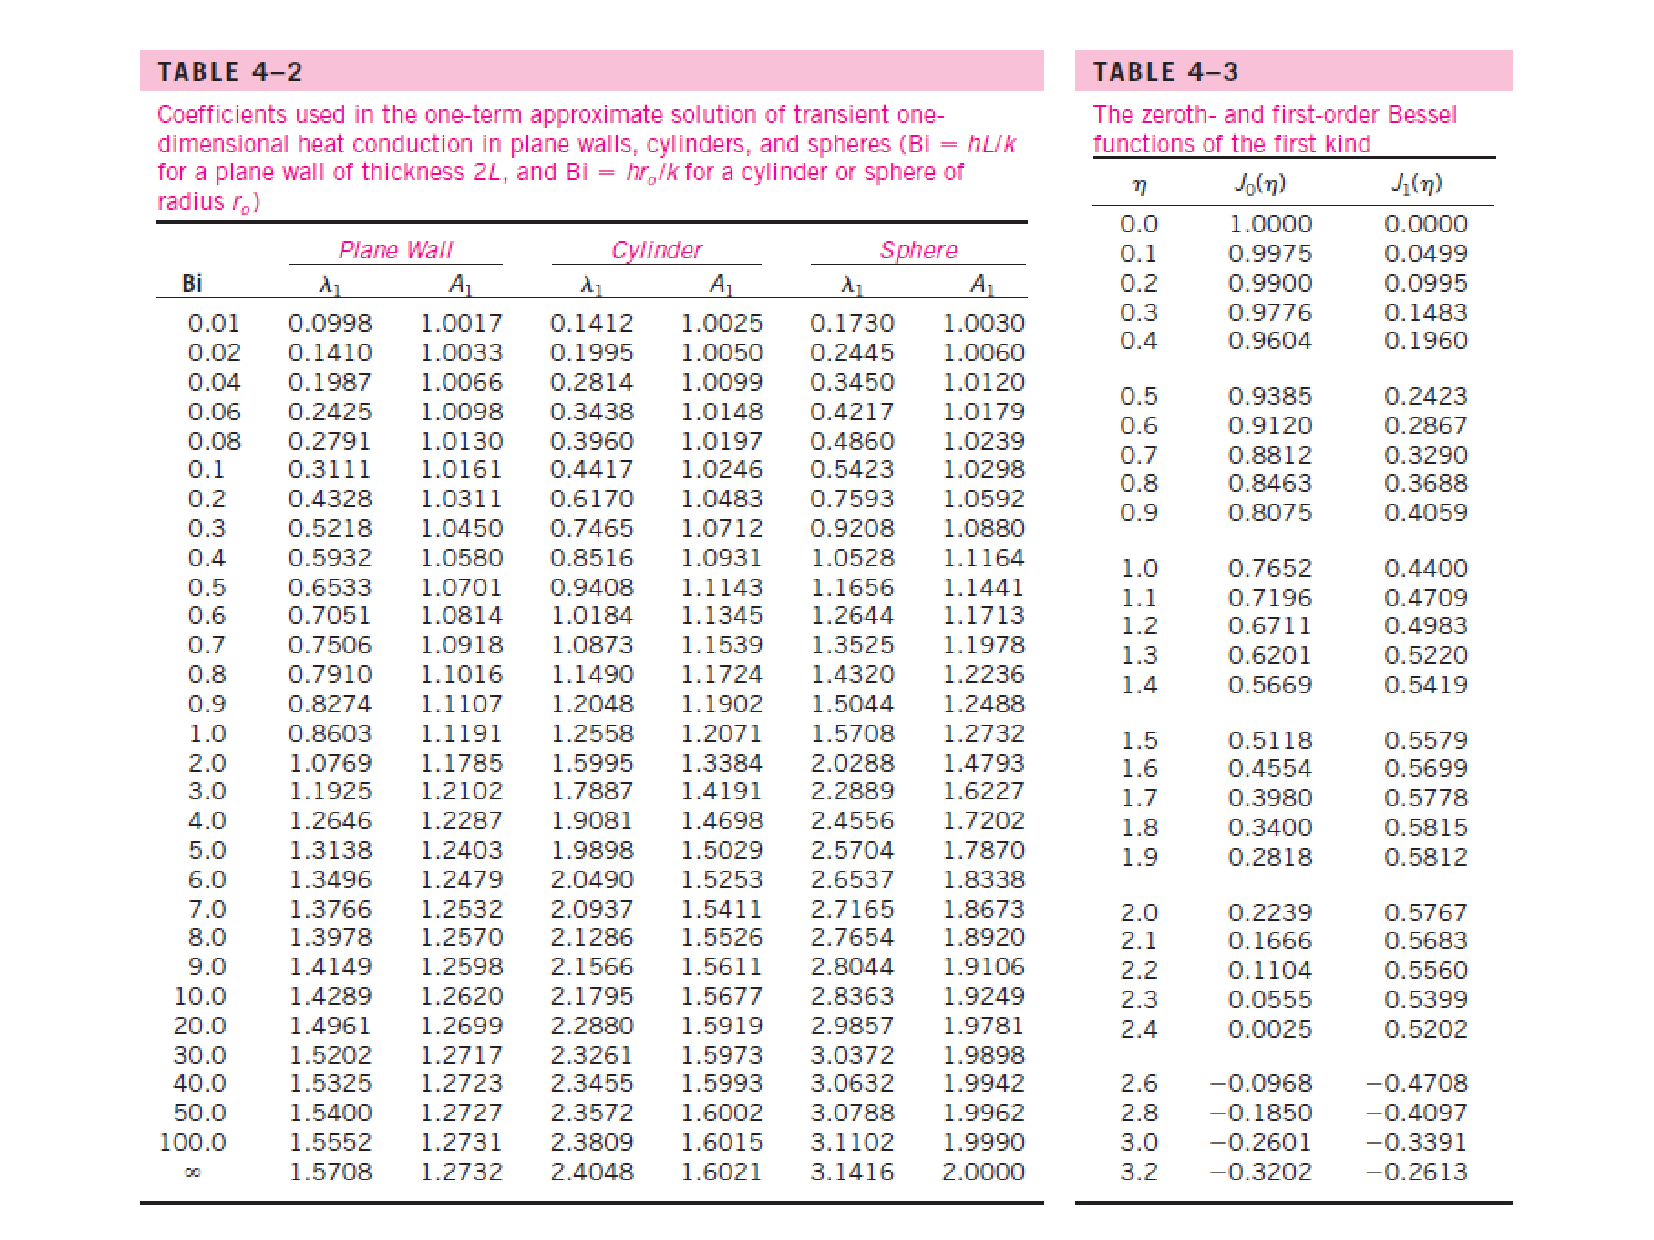
\includepdf{BaselFunctionTable.pdf}
\paperend
\end{document}
